\section{Modular data, topological defects, and conformal boundaries}
\label{sec:physics-defects}

We use the positive spherical structure and the Evans--Gannon ordering
\[
 (0,b,a,c_0,c_1,c_2,d_1,d_2,d_3,d_4,d_5,d_6).
\]
The translation to the labels used in the Haagerup bootstrap literature is
\[
 (1,\pi_1,\pi_2,\sigma_1,\sigma_2,\sigma_3,
   \mu_5,\mu_2,\mu_1,\mu_3,\mu_6,\mu_4).
\]
The final permutation is fixed by the distinct thirteenth-root twists
in \cite[arXiv version~2, Eq.~(30)]{AHKZ}; retaining the same numerical subscripts for
the $d$ and $\mu$ labels would be incorrect.
In particular, $a$ is a simple object of the center, whereas $\alpha$
below denotes the invertible generator of the six-object Haagerup
category. These two objects have different dimensions and different roles.

Put $r=\sqrt{13}$, $d=(3+r)/2$, $s=2+3d$, and
\[
 A=\frac16-\frac1{2r},\qquad B=\frac16+\frac1{2r},\qquad
 u=\frac13,\qquad v=\frac1r.
\]
In blocks of sizes $1,1,4,6$, the complete normalized matrix is
\begin{equation}
 S=\begin{pmatrix}
 A&B&u\mathbf1_4^{\mathsf t}&v\mathbf1_6^{\mathsf t}\\
 B&A&u\mathbf1_4^{\mathsf t}&-v\mathbf1_6^{\mathsf t}\\
 u\mathbf1_4&u\mathbf1_4&C&0\\
 v\mathbf1_6&-v\mathbf1_6&0&D
 \end{pmatrix},
 \qquad
 C=\frac13\begin{pmatrix}
 2&-1&-1&-1\\-1&2&-1&-1\\-1&-1&-1&2\\-1&-1&2&-1
 \end{pmatrix},
 \label{eq:physics-S}
\end{equation}
where
\begin{equation}
 D_{ij}=-\frac2{\sqrt{13}}\cos\frac{2\pi ij}{13},
 \qquad 1\leq i,j\leq6.
 \label{eq:physics-Sd}
\end{equation}
The topological twist matrix and the character matrix are distinct:
\begin{align}
 \Theta&=\operatorname{diag}\left(
 1,1,1,1,e^{2\pi i/3},e^{4\pi i/3},
 e^{2\pi i6/13},e^{2\pi i11/13},e^{2\pi i2/13},
 e^{2\pi i5/13},e^{2\pi i7/13},e^{2\pi i8/13}\right),\\
 T_{\rm ch}&=e^{-2\pi i/3}\Theta.
 \label{eq:physics-T}
\end{align}
Thus the $d_j$ twist is $e^{2\pi i6j^2/13}$. The conformal weight of
$d_3$ is $15/13$, although its twist exponent is $2/13$.
These are the standard positive Haagerup modular data
\cite{EG}; no numerical eigenvector choice enters these formulas.

The categorical dimensions and total quantum dimension are
\begin{equation}
 (\operatorname{qdim}M_i)_i=(1,d^2,s,s,s,s,3d,3d,3d,3d,3d,3d),
 \qquad \mathcal D=\frac1{S_{00}}=3s.
 \label{eq:physics-qdim}
\end{equation}
Here $\mathcal D^2$, rather than $\mathcal D$, is the global dimension
of $\operatorname{Rep}(U)$. Every simple object is self-dual because
$S^2=1$. The six-object Haagerup category has global dimension
$3+3d^2=3s=\mathcal D$.

\begin{figure}[tbp]
 \centering
 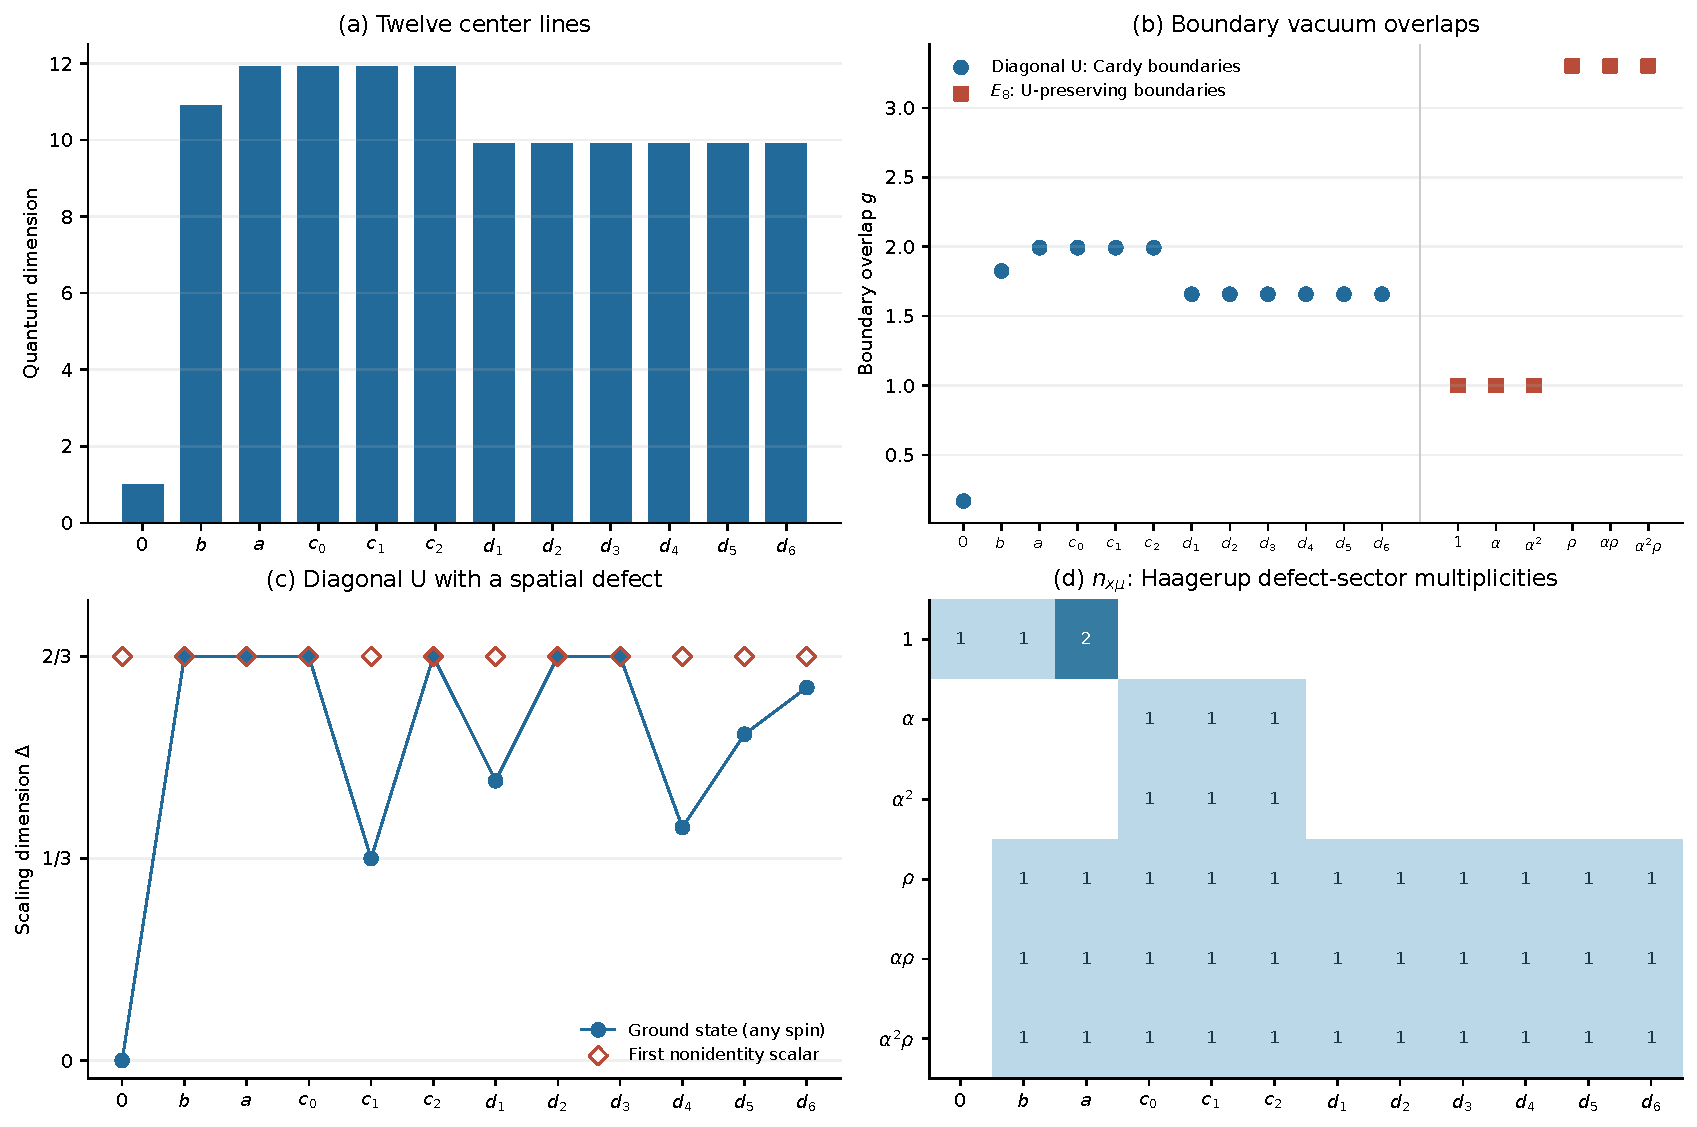
\includegraphics[width=\textwidth]{c8_physics_20260927/figures/defect_observables.pdf}
 \caption{Exact modular and defect observables, displayed using the
 positive embedding of the exported algebraic data. The ground-state
 gap in a twisted space and its scalar gap are distinct; the latter
 is $2/3$ for all twelve diagonal-theory lines. The final panel records
 the integer forgetful multiplicity matrix for the selected extension.}
 \label{fig:physics-defects}
\end{figure}

\subsection{Exact fusion and diagonal-theory defect spectra}

Consider first the diagonal full CFT
\begin{equation}
 \mathcal H_U=\bigoplus_i M_i\otimes\overline{M_i},
 \qquad Z_U(\tau,\bar\tau)=\sum_i|\chi_i(\tau)|^2.
\end{equation}
Its twelve chiral-algebra-preserving Verlinde lines form the fusion
category underlying $\operatorname{Rep}(U)=Z(\mathcal H_3)$.
Their multiplication and their action on bulk sectors are
\begin{equation}
 N_{ab}^{\phantom{ab}c}
   =\sum_i\frac{S_{ai}S_{bi}S_{ci}}{S_{0i}},
 \qquad
 \widehat L_a\big|_{M_i\otimes\overline{M_i}}
   =\lambda_a(i)\,\mathrm{id},
 \qquad \lambda_a(i)=\frac{S_{ai}}{S_{0i}}.
 \label{eq:physics-Verlinde}
\end{equation}
Complex conjugation is absent from the displayed Verlinde sum because
$S$ is real. In particular $\lambda_a(0)=\operatorname{qdim}(M_a)$.
The line insertion and its modular transform give
\begin{align}
 Z_U^{[a]}(\tau,\bar\tau)
   &=\sum_i\lambda_a(i)|\chi_i(\tau)|^2,\\
 Z_{U,[a]}(\tau,\bar\tau)
   &=\sum_{i,j}N_{ai}^{\phantom{ai}j}
           \chi_i(\tau)\overline{\chi_j(\tau)}.
 \label{eq:physics-twisted}
\end{align}
The first expression is a trace with a line operator and its coefficients
need not be positive. The second is the partition function of the Hilbert
space with an $a$ defect intersecting the spatial circle; all its
multiplicities are nonnegative integers. This is the usual distinction
between a twined trace and a twisted Hilbert space \cite{PZ,LS}.
Indeed, applying $S$ to the first expression makes the coefficient of
$\chi_i\overline{\chi_j}$ equal to the sum in
\eqref{eq:physics-Verlinde}, proving the second formula directly.

The attached data give all $1728$ integers $N_{ab}^{\phantom{ab}c}$,
all $144$ line eigenvalues, and all twelve matrices in
\eqref{eq:physics-twisted}. They also give the lowest scaling dimension
and the lowest nonidentity scalar dimension in each twisted space.
For orientation, some compact fusion products are
\begin{align}
 b^2&=1+b+a+\sum_{j=0}^2c_j+\sum_{j=1}^6d_j,\\
 a^2&=1+2b+2a+\sum_{j=0}^2c_j+\sum_{j=1}^6d_j,\\
 d_i^2&=1+a+\sum_{j=0}^2c_j+
                 \sum_{\substack{1\leq j\leq6\\j\ne[2i]}}d_j.
\end{align}
Here $[m]$ is the representative of $\{m,-m\}$ modulo $13$ in
$\{1,\ldots,6\}$. The gap data are particularly simple:
\begin{center}
\begin{tabular}{c|rr|rr}
\toprule
Line&ground $\Delta$&multiplicity&scalar gap&multiplicity\\
\midrule
$0$&$0$&$1$&$2/3$&$9$\\
$b$&$2/3$&$18$&$2/3$&$18$\\
$a,c_0$&$2/3$&$9$&$2/3$&$9$\\
$c_1$&$1/3$&$6$&$2/3$&$18$\\
$c_2$&$2/3$&$63$&$2/3$&$9$\\
$d_1$&$6/13$&$14$&$2/3$&$9$\\
$d_2,d_3$&$2/3$&$9$&$2/3$&$9$\\
$d_4$&$5/13$&$10$&$2/3$&$9$\\
$d_5$&$7/13$&$26$&$2/3$&$9$\\
$d_6$&$8/13$&$28$&$2/3$&$9$\\
\bottomrule
\end{tabular}
\end{center}
The scalar condition is $h=\bar h$, not merely integral spin.
For a summand $M_i\otimes\overline{M_j}$ it first requires
$h_i-h_j\in\mathbb Z$. Among the supplied lowest weights the only
unequal pair with this property is $0$ versus $1$; its scalar ground
states use $U_1$ on the vacuum side. Consequently all the reported
lowest scalar multiplicities follow from the twelve top dimensions and
$\dim U_1=6$, without an extrapolation of character coefficients.

A useful symmetry test follows immediately from invertibility of $S$.
If a bulk sector $i$ is fixed by every line, its eigenvalues must obey
$\lambda_a(i)=\lambda_a(0)$ for every $a$. The $i$th column of $S$
would then be proportional to the vacuum column; hence $i=0$.
Thus the fully Verlinde-invariant space is
$U\otimes\overline U$. Its first nonidentity scalars have weights
$(1,1)$ and multiplicity $6^2=36$. Its scalar gap is $2$, even though
the unrestricted diagonal theory has scalar gap $2/3$.

\subsection{Cardy boundaries and their annuli}

The diagonal theory has twelve elementary boundaries preserving $U$.
With the usual normalized Ishibashi states, Cardy's solution reads
\begin{equation}
 |a\rangle=\sum_i\frac{S_{ai}}{\sqrt{S_{0i}}}|i\rangle\!\rangle,
 \qquad
 Z_{ab}^{\rm open}(q)=\sum_iN_{ab}^{\phantom{ab}i}\chi_i(q).
 \label{eq:physics-Cardy}
\end{equation}
All labels are self-dual, so no conjugate label is needed in the annulus
formula. Modular transformation of the closed-channel overlap gives
the same Verlinde sum as above, providing a direct check of the open
channel multiplicities \cite{Cardy}.

The boundary vacuum overlaps, conventionally denoted by $g_a$, are
\begin{equation}
 g_a=\frac{S_{a0}}{\sqrt{S_{00}}}
     =\frac{\operatorname{qdim}(M_a)}{\sqrt{3s}},
 \qquad \log g_a\ \text{is the boundary entropy}.
 \label{eq:physics-g}
\end{equation}
They therefore take four values, in the proportions
$1:d^2:s:3d$. The exact squared values lie in $\mathbb Q(\sqrt{13})$;
the dataset supplies these as exact algebraic numbers as well as
decimal values of $g_a$ for plotting. The $144$ annulus entries include
the identity multiplicity, the lowest boundary weight, and the first
positive boundary weight. The last quantity includes weight-one
currents in the vacuum representation. Removing the entire vacuum
representation would define a different gap.
For the vacuum Cardy boundary the first positive boundary weight is
$1$, with six currents. Every other elementary Cardy boundary has
boundary-preserving fields of weight $1/3$; there are six for boundary
$c_1$ and three for each of the other ten boundaries. These are relevant
boundary perturbations, without implying a particular endpoint of
their renormalization-group flows.

\section{The Haagerup symmetry of the holomorphic extension}
\label{sec:physics-H3}

The twelve diagonal-theory lines above must be distinguished from the
six Haagerup lines obtained after extension. Let
$H'=V_{E_8}$ be the selected holomorphic extension, with underlying
$U$-module
\begin{equation}
 H'\big|_U\simeq M_0\oplus M_b\oplus2M_a,
 \qquad \chi_{E_8}=\chi_0+\chi_b+2\chi_a.
 \label{eq:physics-E8-extension}
\end{equation}
Its algebra object is denoted by $A$, and
$\mathcal C=\operatorname{Rep}(U)_A\simeq\mathcal H_3$ is the
category of all right $A$-modules, including the nonlocal ones.
The local $A$-module category is trivial. The six simples of
$\mathcal C$ are $1,\alpha,\alpha^2,\rho,\alpha\rho,\alpha^2\rho$,
with
\begin{equation}
 \alpha^3=1,\qquad \rho\alpha=\alpha^2\rho,\qquad
 \rho^2=1+\rho+\alpha\rho+\alpha^2\rho.
 \label{eq:physics-H3-ring}
\end{equation}
The full $E_8$ theory has the corresponding
$\mathcal C\boxtimes\mathcal C^{\rm op}$ defects. In this section
we select the first factor, leaving the antiholomorphic $H'$ theory as
a spectator. This convention specifies a single $\mathcal H_3$ action
to which the twelve-sector Haagerup bootstrap applies.

\subsection{Forgetful multiplicities and the physical sector assignment}

Under the center equivalence
$\operatorname{Rep}(U)\simeq Z(\mathcal C)$, the free-module functor
is the central forgetful functor $F:Z(\mathcal C)\to\mathcal C$.
Writing $X=\rho\oplus\alpha\rho\oplus\alpha^2\rho$, its values are
\begin{equation}
 F(0)=1,\quad F(b)=1\oplus X,\quad F(a)=2\cdot1\oplus X,
 \quad F(c_j)=\alpha\oplus\alpha^2\oplus X,
 \quad F(d_j)=X.
 \label{eq:physics-forgetful}
\end{equation}
These are the Haagerup branching rules of
\cite[Eq.~(4.49)]{LOST}. They specify the entire $6\times12$ matrix
$n_{x\mu}=\dim\operatorname{Hom}_{\mathcal C}(F(M_\mu),x)$.
For example its first three rows are
\begin{align}
 n_1&=(1,1,2,0,0,0,0,0,0,0,0,0),\\
 n_\alpha=n_{\alpha^2}&=(0,0,0,1,1,1,0,0,0,0,0,0),
\end{align}
and each of the other three rows is
$(0,1,1,1,1,1,1,1,1,1,1,1)$.

Here is an intrinsic reason for the sector identification, beyond a
check of modular covariance. If $R$ is restriction of an $A$-module
to $U$, free--forgetful adjunction gives
\begin{equation}
 \operatorname{Hom}_{U}(M_\mu,Rx)
 \simeq\operatorname{Hom}_{\mathcal C}(F(M_\mu),x),
 \qquad
 Rx\simeq\bigoplus_\mu n_{x\mu}M_\mu.
 \label{eq:physics-adjunction}
\end{equation}
In the standard rational-CFT construction of the selected first-factor
defects, their Hilbert spaces are $Rx\otimes\overline{H'}$.
The tube-algebra decomposition is therefore
\begin{equation}
 \mathcal H_x
  \simeq\bigoplus_\mu W_x^\mu\otimes\mathcal V_\mu,
 \qquad
 W_x^\mu=\operatorname{Hom}_{\mathcal C}(F(M_\mu),x),
 \qquad
 \mathcal V_\mu=M_\mu\otimes\overline{H'}.
 \label{eq:physics-tube-space}
\end{equation}
This is the multiplicity-space convention of
\cite[Eq.~(4.1)]{LS}. A full tube-projector image also contains the
finite-dimensional factor $W_x^\mu$; it is not in general a single
copy of $\mathcal V_\mu$. In particular $\dim W_1^a=2$.
The physical interpretation in \eqref{eq:physics-tube-space} uses the
canonical extension and its rational-CFT defect construction; modular
covariance alone would not establish that interpretation for an
arbitrary vector-valued function.

It follows that the twelve bootstrap partition functions and the six
twisted Hilbert-space partition functions are
\begin{equation}
 Z_\mu^{3d}(\tau,\bar\tau)
   =\chi_\mu(\tau)\overline{\chi_{E_8}(\tau)},
 \qquad
 Z_x(\tau,\bar\tau)=\sum_\mu n_{x\mu}Z_\mu^{3d}(\tau,\bar\tau).
 \label{eq:physics-H3-sector-functions}
\end{equation}
For $x=1$, \eqref{eq:physics-E8-extension} recovers
$Z_1=|\chi_{E_8}|^2$. Since $\chi_{E_8}$ is $S$-invariant and has
$T$ multiplier $e^{-2\pi i/3}$, these functions transform by
$(S,\Theta)$: the left and right central-charge phases cancel.
This also checks the spin convention used in the bootstrap.

\subsection{Untwisted charges and scalar gaps}

On the three untwisted multiplicity factors, one may choose bases in
which the line actions are
\begin{equation}
 \begin{array}{c|cc}
   &\widehat\alpha&\widehat\rho\\\hline
   M_0&1&d\\
   M_b&1&-d^{-1}\\
   \mathbb C^2\otimes M_a&
    \begin{pmatrix}\omega&0\\0&\omega^2\end{pmatrix}&
    \begin{pmatrix}0&1\\1&0\end{pmatrix}
 \end{array}
 \qquad \omega=e^{2\pi i/3}.
 \label{eq:physics-H3-action}
\end{equation}
The matrices obey \eqref{eq:physics-H3-ring}; for the two-dimensional
block the three noninvertible matrices sum to zero, so $\rho^2=1$ on
that block is consistent with the categorical fusion rule.
The resulting first-factor twined traces include
\begin{align}
 Z^{[\alpha]}&=(\chi_0+\chi_b-\chi_a)\overline{\chi_{E_8}},\\
 Z^{[\rho]}&=(d\chi_0-d^{-1}\chi_b)\overline{\chi_{E_8}}.
 \label{eq:physics-H3-twined}
\end{align}
They act trivially on the antiholomorphic factor. Squaring their
holomorphic factors in absolute value instead would correspond to
particular paired left/right insertions, rather than the selected
first-factor action.

Every antiholomorphic $E_8$ weight is an integer. Thus the sectors
$c_1,c_2,d_1,\ldots,d_6$ in
\eqref{eq:physics-H3-sector-functions} contain no scalar states at
any grade. Their nonintegral left weights cannot equal an integer
right weight. The remaining sectors $0,b,a,c_0$ have their first
nonidentity scalars at $(h,\bar h)=(1,1)$:
\begin{equation}
 \begin{array}{c|rrrr}
 \mu&0&b&a&c_0\\\hline
 \Delta_{\rm scalar}&2&2&2&2\\
 \text{multiplicity in }\mathcal V_\mu&6\cdot248&80\cdot248&81\cdot248&81\cdot248.
 \end{array}
 \label{eq:physics-H3-scalar-table}
\end{equation}
The $\mathcal H_3$-invariant scalar gap is therefore $2$, and so is
the scalar gap in $\mathcal V_{\pi_2}\cup\mathcal V_{\sigma_1}$.
The physical untwisted $\mathbb Z_3$-charged space contains two copies
of $\mathcal V_{\pi_2}$, with scalar multiplicity $2\cdot81\cdot248$.
The union used in the bootstrap is a union of tube multiplicity spaces;
it must not be identified with that entire untwisted charged space.

\subsection{Six boundaries of the extended theory}

The same module category supplies six elementary boundaries of the full
$E_8$ theory which preserve $U$. For $x,y\in\mathcal C$, their open
state space is $R(x^*\otimes_A y)$, hence
\begin{equation}
 Z^{E_8,\mathrm{open}}_{xy}(q)
  =\sum_{z,\mu}N_{x^*y}^{\phantom{x^*y}z}
                  n_{z\mu}\chi_\mu(q).
 \label{eq:physics-E8-annuli}
\end{equation}
The invertible duals are $\alpha^*=\alpha^2$; the three noninvertible
objects are self-dual. This dual must be retained in the annulus formula,
even though it could be omitted for the twelve self-dual center labels.

The normalization of the boundary entropy can be derived without an
unknown proportionality constant. Restriction multiplies categorical
dimensions by $\operatorname{qdim}(A)=\mathcal D$, so the coefficient
of the vacuum in the modular transform of
\eqref{eq:physics-E8-annuli} is
\[
 S_{00}\operatorname{qdim}_{\operatorname{Rep}(U)}
       R(x^*\otimes_A y)
 =\operatorname{qdim}_{\mathcal C}(x)
       \operatorname{qdim}_{\mathcal C}(y).
\]
Reflection positivity chooses the positive overlaps. Thus
\begin{equation}
 (g_1,g_\alpha,g_{\alpha^2},g_\rho,g_{\alpha\rho},g_{\alpha^2\rho})
   =(1,1,1,d,d,d).
 \label{eq:physics-E8-g}
\end{equation}
In particular the ordinary $E_8$ boundary has $g_1=1$ and self-annulus
$\chi_{E_8}$. Its first positive boundary weight is $1$, with $248$
currents. The same holds for the other two invertible boundaries.
Each noninvertible boundary instead has nine fields of weight $1/3$
in its self-annulus. Between distinct noninvertible boundaries there
are twelve ground fields of weight $1/3$; between two distinct
invertible boundaries, or an invertible and a noninvertible boundary,
there are three. All $36$ annuli and their exact $g$ values are supplied.

\subsection{What the attached exact data check}

The exporter \path{c8_physics_20260927/defects.py} works in
$\mathbb Q(\zeta_{13})$ and represents every field element by twelve
rational coefficients. Its square root is the explicit Gauss sum
\[
 \sqrt{13}=\sum_{j=1}^{12}\left(\frac j{13}\right)\zeta_{13}^j.
\]
It checks $S^2=1$, $(S\Theta)^3=1$, exact nonnegative integrality of
all Verlinde coefficients, associativity, and multiplicativity of
dimensions. The $6\times12$ forgetful table is independently checked
as a based-ring homomorphism, and its vacuum row is checked to be
$S$- and $\Theta$-invariant. No coefficient is inferred by rounding.
Decimal columns serve only as plot coordinates.
The guarded run completed all these checks successfully; the saved
JSON includes the generator hash and the precise normalization of
every exported array.

The output files contain the complete fusion, line, annulus, twisted,
and tube-sector recipes. These checks verify consequences of the
given modular data and character tops. They neither replace the
construction of $U$ nor reconstruct associators, braidings, or
operator-product coefficients from modular data alone.
